\chapter{Ulteriori argomenti}
\section{Marce aleatorie (random walks)}
\begin{Definition}{Marcia aleatoria semplice simmetrica}{}
    Sia $Z_0, Z_1, Z_2,...$ una sequenza di variabili aleatorie i.i.d. tali che:
    \begin{align*}
        P(Z_i=1)&=\frac{1}{2}\\
        P(Z_i=-1)&=\frac{1}{2}
    \end{align*}
    la sequenza di variabili aleatorie $S_0, S_1, S_2, ...$ dove $S_0=0$ con probabilità 1 e $\forall n>0$ $S_n=\sum^n_{i=1}Z_i$ si dice marcia aleatorie semplice simmetrica.
\end{Definition}

\begin{figure}[h]
    \centering
    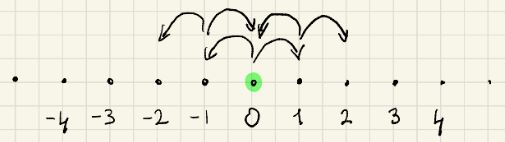
\includegraphics[width=0.5\linewidth]{images/marcia-aleatoria.JPG}
    \caption{Marcia aleatoria}
    \label{fig:marcia-aleatoria}
\end{figure}

$S_n$ è la posizione al passo $n$ e ad ogni passo saltiamo a destra con probabilità $\frac{1}{2}$ e a sinistra con probabilità $\frac{1}{2}$. Le variabili aleatorie $Z_1,Z_2,...$ si dicono incrementi della marcia aleatoria $S_0, S_1, S_2,...$

\begin{Definition}{Marcia aleatoria semplice}{}
    Sia $Z_0, Z_1, Z_2, ...$ una sequenza di variabili aleatorie i.i.d. tali che:
    \begin{align*}
        P(Z_i=1)&=p\\P(Z_i=-1)&=1-p
    \end{align*}
    dove $p\in(0,1)$. La sequenza di variabili aleatorie $S_0, S_1, S_2, ...$ dove $S_0=0$ con probabilità 1 e $S_n=\sum^n_{i=1}Z_i$ si dice marcia aleatoria semplice.
\end{Definition}

Se $p=\frac{1}{2}$ otteniamo la marcia aleatoria semplice simmetrica, se $p\neq\frac{1}{2}$ la marcia aleatoria semplice asimmetrica.

\begin{Example}{Marcia aleatoria}{}
    \textit{Consideriamo una marcia aleatoria simmetrica, $S_0, S_1, S_2, ...$ utilizzare il teorema limite centrale per approssimare la probabilità che al passo $n$ la marcia si trovi nell'intervallo $[a\sqrt{n}, b\sqrt{n}]$, per $a<b$ e valori sufficientemente grandi di $n$, dove si trova $5n$ e con quale probabilità?}

    \begin{align*}
        P(a\sqrt{n}\leq S_n\leq b\sqrt{n})=\sum_{i\in Z}P(S_n=i)=\\\sum_{i\in Z, i\leq b\sqrt{n}}P(S_n=i)-P_{i\in Z, i<a\sqrt{n}}(S_n=1)=P(S_n\leq b\sqrt{n})-P(S_n<a\sqrt{n})
    \end{align*}
    \begin{align*}
        \mu&=E(Z_i)=1P(Z_i=1)+(-1)P(Z_i=-1)=\frac{1}{2}-\frac{1}{2}=0\\
        \sigma&=\sqrt{Var(Z_i)}=\sqrt{E(Z_i^2)-E(Z_i)^2}=\sqrt{1^2-0^2}=1
    \end{align*}
    \begin{align*}
        P(S_n\leq b\sqrt{n})=P\left(\frac{(\sum^n_{i=1})-\mu n}{\sigma\sqrt{n}}\leq \frac{b\sqrt{n}-\mu n}{\sigma\sqrt{n}}\right)=P(a\sqrt{n}\leq S_n\leq b\sqrt{n})\approx\Phi(b)-\Phi(a)=\\P(-3\sqrt{n}\leq S_n\leq 3\sqrt{n})\approx\Phi(3)-\Phi(-3)=2\Phi(3)-1\approx 0.9974
    \end{align*}
\end{Example}

\begin{Definition}{Marcia aleatoria}{}
    Sia $Z_0, Z_1, Z_2, ...$ una sequenza di variabili aleatoria i.i.d. con valori in $I=Z$ e densità $p(i)$.

    La sequenza $S_0, S_1, ...$ con $S_0=0$ con probabilità 1 e $S_n=\sum^n_{i=1}Z_i$ si dice marcia aleatoria.
\end{Definition}

\section{Catene di Markov}


Per una catena di Markov abbiamo bisogno di:
\begin{enumerate}
    \item un'insieme di stati $I=\{1,2,3,...,j\}$ (i punti in cui la marcia si può trovare ad ogni passo);
    \item una matrice $kxk$ $P=(p_{i,j})_{i,j\in I}$, con $p_{i,j}\in[0,1]$ e $\sum_{j=1}^Ip_{i,j}=1$ (la somma su tutti gli elementi di qualsiasi riga $i$ deve fare 1). Tale matrice si dice \textit{stocastica}.
\end{enumerate}

Dato un'insieme di stati e una matrice stocastica $P=(p_{i,j})_{i,j\in I}$ rappresentiamo un grafo come segue:
\begin{enumerate}
    \item i punti (vertice del grafo) sono gli stati, cioè gli elementi di $I$;
    \item colleghiamo ogni stato $i$ con ogni stato $j$ con una freccia diretta da $i$ a $j$ (arco) se $p_{i,j}>0$.
\end{enumerate}

\begin{Definition}{Catena di Markov}{}
    La catena di Markov è una sequenza di variabili aleatorie $S_0, S_1, S_2, S_3, ...$ tale che:
    \begin{equation*}
        \forall n\in \mathbb{N}\mbox{ e }i,j\in I\hspace{1cm}P(S_{n+1}=j|S_n=i)=p_{i,j}
    \end{equation*}
    dove $P=(p_{i,j})_{i,j\in I}$ è una matrice stocastica e $I$ è l'insieme degli stati.
\end{Definition}

\begin{Thm}{Catena di Markov}{}
    Sia $S_0, S_1, ..., S_n$ una catena di Markov con spazio degli stati $I=\{1,2,3,...,k\}$ che parte dallo stato $l\in I$. Allora $\forall j\in I$, $\forall n\in \mathbb{N}$, $\forall r\in\mathbb{N}$:
    \begin{equation*}
        P(S_n=j)P(S_{r+n}=j|S_r=l)=(P^n)_{l,j}
    \end{equation*}
    sapendo che la matrice stocastica è $P(p_{i,j})_{i,j\in I}$ dove $P^n$ è la matrice $P$ moltiplicata $n$ volte con se stessa e $(P^n)_{i,j}$ è la sua componente $i,j\in I$.
\end{Thm}

\begin{figure}
    \centering
    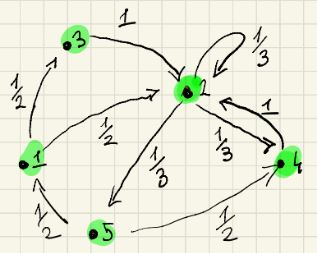
\includegraphics[width=0.5\linewidth]{images/catena-di-markov.JPG}
    \caption{Catena di Markov}
    \label{fig:catena-di-markov}
\end{figure}

\begin{Example}{Catena di Markov}{}
    \textit{Un server è in uno stato $I$ (inattivo) o $A$ (attivo). Ogni secondo il suo stato viene aggiornato. Se il server è attivo, esso diventa inattivo con probabilità $\alpha$. Se il server è inattivo, esso diventa attivo con probabilità $\beta$. Determinare la probabilità che esso sia nello stato attivo dopo 2 secondi supponendo che esso parte dallo stato inattivo.}

    \begin{minipage}{\textwidth}
        \centering
        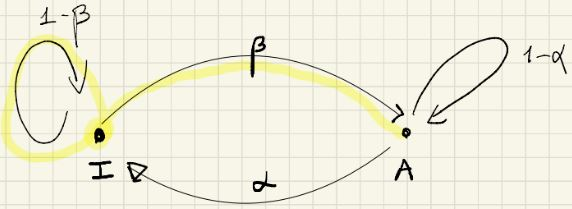
\includegraphics[width=0.6\linewidth]{images/esempio-catena-markov.JPG}
        %\captionof{figure}{Esempio catena di Markov}
    \end{minipage}\\

    \begin{equation*}
        P=\begin{pmatrix}1-\beta & \beta\\\alpha & 1-\alpha\end{pmatrix}
    \end{equation*}
    \begin{equation*}
        p_{1,1}=1-\beta\hspace{1cm}p_{1,2}=\beta\hspace{1cm}p_{2,1}=\alpha\hspace{1cm}p_{2,2}=1-\alpha\hspace{1cm}(P^2)_{1,2}=?
    \end{equation*}
    \begin{equation*}
        \begin{pmatrix}1-\beta & \beta\\\alpha & 1-\alpha\end{pmatrix}\begin{pmatrix}1-\beta & \beta\\\alpha & 1-\alpha\end{pmatrix}=\begin{pmatrix}(1-\beta)^2+\beta\alpha & (1-\beta)\beta+\beta(1-\alpha)\\\alpha(1-\beta)+\alpha(1-\alpha) & \alpha\beta+(1-\alpha)^2\end{pmatrix}
    \end{equation*}
    \begin{equation*}
        (P^2)_{1,2}=(1-\beta)\beta+\beta(1-\alpha)
    \end{equation*}
\end{Example}